\documentclass[10pt]{beamer}

\usepackage[brazilian]{babel}
\usepackage[utf8]{inputenc}
\usepackage{graphicx}
\usepackage{mathtools}
\usepackage{amsthm}
\usepackage{thmtools,thm-restate}
\usepackage{amsfonts}
\usepackage{hyperref}
\usepackage[singlelinecheck=false]{caption}
\usepackage[backend=biber,url=true,doi=true,eprint=false,style=alphabetic]{biblatex}
\usepackage[justification=centering]{caption}
\usepackage{indentfirst}
\usepackage{enumitem}
\usepackage{algorithm}
\usepackage{algpseudocode}
\usepackage{listings}
% Timeline
\usepackage{xcolor}
\newcommand\ytl[2]{
\parbox[b]{8em}{\hfill{\color{cyan}\bfseries\sffamily #1}~$\cdots\cdots$~}\makebox[0pt][c]{$\bullet$}\vrule\quad \parbox[c]{7.5cm}{\vspace{2pt}\color{red!40!black!80}\raggedright\sffamily #2.\\[7pt]}\\[-3pt]}

% Fix beamer and enumitem conflicts.
\setitemize{label=\usebeamerfont*{itemize item}%
  \usebeamercolor[fg]{itemize item}
\usebeamertemplate{itemize item}}

% Remove line breaks.
\setbeamertemplate{bibliography entry title}{}
\setbeamertemplate{bibliography entry location}{}
\setbeamertemplate{bibliography entry note}{}

\uselanguage{Brazilian}
\languagepath{Brazilian}
\usetheme{Berlin}

\addbibresource{references.bib}

\newcommand\nmfootnote[1]{%
  \begingroup
  \renewcommand\thefootnote{}\footnote{#1}%
  \addtocounter{footnote}{-1}%
  \endgroup
}

\makeatletter
\def\subsection{\@startsection{subsection}{3}%
  \z@{.5\linespacing\@plus.7\linespacing}{.1\linespacing}%
  {\normalfont}}
\makeatother

\DeclareMathOperator*{\argmin}{arg\,min}
\DeclareMathOperator*{\argmax}{arg\,max}

\newcommand\defeq{\mathrel{\overset{\makebox[0pt]{\mbox{\normalfont\tiny\sffamily def}}}{=}}}

\floatname{algorithm}{Algoritmo}
\algrenewcommand\algorithmicrequire{\textbf{Input}}
\algrenewcommand\algorithmicensure{\textbf{Output}}

\captionsetup[table]{labelsep=space}

\theoremstyle{plain}

\newtheorem{proposition}{Proposição}
\newtheorem{exercise}{Exercício}

\newcommand{\set}[1]{\mathbf{#1}}
\newcommand{\pr}{\mathbb{P}}
\renewcommand{\implies}{\Rightarrow}

\newcommand{\bigo}{\mathcal{O}}
\newcommand{\p}{\pause}

\setlength{\parskip}{1em}

\lstset{frameround=fttt,
  language=[5.3]Lua,
  numbers=left,
  breaklines=true,
  keywordstyle=\bfseries,
  basicstyle=\ttfamily,
}

\newcommand\Fontsmall{\fontsize{12}{7.2}\selectfont}

\newcommand{\code}[1]{\lstinline[mathescape=true]{#1}}
\newcommand{\mcode}[1]{\lstinline[mathescape]!#1!}

\title{GNU Hurd}
\subtitle{MAC0422 --- Estudo de Caso}
\author{Renato Lui Geh}

\begin{document}

\frame{\titlepage}

\begin{frame}
  \frametitle{Índice}
  \tableofcontents
\end{frame}

%--------------------------------------------------------------------------------------------------

\section{História}

\begin{frame}
  \frametitle{História do GNU/Hurd}

  \begin{table}
    \begin{minipage}[t]{\linewidth}
      \color{gray}
      \rule{\linewidth}{1pt}
      \ytl{1983}{Richard Stallman (RMS) cria o projeto GNU}
      \ytl{1986}{RMS decide usar o TRIX como kernel}
      \ytl{1988}{É decidido usar o Mach como kernel}
      \ytl{1991}{GNU Hurd é anunciado ao público}
      \ytl{1994}{Primeiro boot}
      \ytl{1994}{Emacs e gcc rodam pela primeira vez}
      \ytl{1995}{ext2fs, ftp}
      \ytl{1996}{NFS e GNU Hurd 0.1}
      \ytl{1997}{GNU Hurd 0.2}
      \bigskip
      \rule{\linewidth}{1pt}
    \end{minipage}
  \end{table}

\end{frame}

\begin{frame}
  \frametitle{História do GNU/Hurd}

  \begin{table}
    \begin{minipage}[t]{\linewidth}
      \color{gray}
      \rule{\linewidth}{1pt}
      \ytl{2011}{GNU Hurd 0.4}
      \ytl{2013}{Debian GNU/Hurd, GNU Hurd 0.5}
      \ytl{2015}{GNU Hurd 0.6}
      \ytl{2016}{GNU Hurd 0.8}
      \rule{\linewidth}{1pt}
    \end{minipage}
  \end{table}
  \begin{figure}[h]
    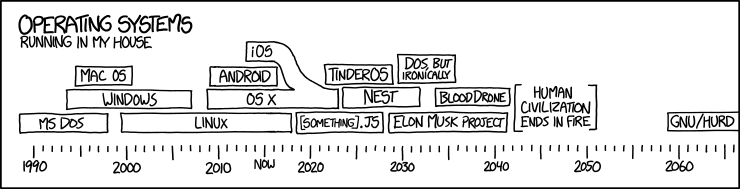
\includegraphics[scale=0.4]{imgs/xkcd_1508.png}
    \caption{\url{https://xkcd.com/1508/}}
  \end{figure}
\end{frame}

\begin{frame}[fragile]
  \frametitle{GNU HURD}

  HURD: Hird of Unix-Replacing Daemons

  HIRD: Hurd of Interfaces Representing Depth

  \begin{lstlisting}[mathescape=true,showstringspaces=false,numbers=none,frame=single]
  GNU HURD := [
    GNU  := GNU's Not Unix
    HURD := [
      HIRD := [
        HURD := [
          $\ldots$
        ] of Interfaces Representing Depth
      ] of Unix-Replacing Daemons
    ]
  ]
  \end{lstlisting}

\end{frame}

\section{Arquitetura Geral}

\begin{frame}
  \frametitle{Arquitetura do GNU Hurd}

  \begin{itemize}
    \item Microkernel (Mach)
    \item Multiservidor
    \item GNU C
    \item Servidores flexíveis (nível usuário)
    \item Servidores compilados como quiser
    \item MIG (Mach Interface Generator)
  \end{itemize}
\end{frame}

\section{Microkernel/Mach}



\section{Memória}

\section{Escalonamento de Processos}

\section{Sistema de Arquivos}

\section{Cache e TLB}

\section{Comparação}

%--------------------------------------------------------------------------------------------------

\section[Referências]{Referências e Bibliografia}
\begin{frame}[t,allowframebreaks]
  \frametitle{Referências e Bibliografia}
  \footnotesize
  \nocite{*}
  \printbibliography[]
\end{frame}

\end{document}
